% The main LaTeX file for the NexusWide StyleGuide PDF documentations.


\documentclass[13pt]{scrarticle}


% text_formatting_oriented_packages.
\usepackage[utf8]{inputenc}
\usepackage[english]{babel}
\usepackage{microtype}
\usepackage[none]{hyphenat}
\usepackage{parskip}
\usepackage[onehalfspacing]{setspace}
%


% graphical_formatting_oriented packages.
\usepackage{graphicx}
\usepackage[cc]{titlepic}
\usepackage{fancyhdr}
\usepackage{tikzsymbols}
\usepackage{xcolor}
%


%
\newcommand{\header}[1]{ \textsf{#1} \relax{}}
\newcommand{\important}[1]{\textit{#1}}
\newcommand{\name}[1]{{\textsc{#1}}}
\newcommand{\nexusrule}[1]{\Tribar[2][white][yellow][brown]{\hspace{0.5cm}#1}}
\newcommand{\example}[1]{{\color{red}$\rangle\hspace{0.3cm} \underline{e.x: }$ \bfseries: ( #1 )}}
%


%
\setlength{\parindent}{0cm}
\widowpenalties 1 1000
\clubpenalties 1 1000
\interlinepenalty 1000


\renewcommand{\familydefault}{\sfdefault}
\renewcommand{\headrulewidth}{0.1cm}
\renewcommand{\footrulewidth}{0.1cm}
%


%
\title{NexusWide Conventions And Regulations Guidelines}
\author{Nima Bavar}
\date{\today}
\titlepic{\parbox{13cm}{
\includegraphics[width=13cm]{/home/nimabavar/Desktop/work/diary/projects/nexus_wide/repositories/style_guide/attachments/nexus_wide_logo.png}}}
%


\begin{document}
    \raggedright
    \pagestyle{fancy}
    \pagenumbering{gobble}

    \fancyhf{}

    \lhead{\leftmark}
    \rhead{\rightmark}
    \rfoot{\thepage}


    \thispagestyle{empty}
    \pagecolor{white}


    \thispagestyle{empty}
    \maketitle{}


    \newpage
    \thispagestyle{fancy}
    \pagenumbering{gobble}
    \setcounter{page}{2}

    \section*{\header{\copyright opyright}}
    \thispagestyle{empty}

    \raggedright
    The corresponding documentation literature and all the containment's, are certified under the \name{Creative Commons Zero v1.0 Universal License} ,
    with the elucidation of the actuality that all branches of \name{modification}, \name{distribution}, \name{patent}, \name{commercial } and \name{private usage } are entirely authorized.
    \newline

    This fragment of dossier is submitted \important{AS IS},
    you are liberate to manufacture any category of modifications you find essential for your individuality or organization.
    \newline

    However, this aforementioned fact loose the \name{NexusWide } team from any fork of provisioned liability or warranty regarding the usage scenario of such composition,
    denoting that we are not held accountable for whichever harm caused by the employment/misemployment of this attestation in any form,
    therefore we demand you to cautiously study the above-mentioned license sanctions if the decision for calibrating this file in a
    personal or officially concealed environment was made. \newline

    The \name{NexusWide } research team welcomes all enhancement ideations announced or pushed to the official repository of the imminent writing.
    \newline


    \newpage
    \thispagestyle{empty}
    \pagenumbering{Roman}


    \begin{centering}
        \vspace*{7cm}
      
        \hspace{1.0cm}
        Dedicated to all the computation enthusiastics \newline
        \hspace*{2.5cm}
        and \newline
        \hspace{0.3cm}
        \name{Free and Open Source Software } producers around the globe.

    \end{centering}


    \newpage
    \pagenumbering{roman}
    \thispagestyle{fancy}
    \setcounter{page}{4}


    \tableofcontents


    \newpage
    \thispagestyle{fancy}
    \pagenumbering{arabic}
    \setcounter{page}{1}

    \section{\header{Conventions}}

    Numerous conventions are globally used throughout this document
    in order to draw attention or to cite particular meanings,
    which are stated in the posterior table:


    \vspace*{2cm}
    \begin{tabular}{r l}

        \hspace{2.8cm}
        \raggedright \textbf{\Large Emphasization} & \textbf{\Large definition} \tabularnewline

        \nexusrule{Text with Tribar} & Nexusrule \tabularnewline
        \example{Red bold text with angle sign} & Rule example \tabularnewline
        \name{small caps text} & Name \tabularnewline
        \important{Italic text} & Important Signification

    \end{tabular}
    \vspace*{2cm}

    The acknowledgment of the aforementioned elements shall be enough
    for you to be prepared to start reading this documentation. \newline

    Do not hesitate to reach out to this table anytime you have forgave the reason behind a specific emphasizing regularity. \newline


    \newpage
    \section{\header{Preface}}


    \name{Durability } and \name{consistency } are the two most prominent chunk of a bested project management course,
    and no project is capable of achieving satisfactory outcomes without proper administration. \newline

    One branch of behavior that can further advance durability by obligating consistency in the best feasible manner,
    is including consequential regulations and laws,
    which is preserved by affixing sharp style guides to the association. \newline

    Thereby to achieve pleasing result in order to avail the esteem and sagacious community of \name{FOSS}\footnote{Free and Open and Source Software.} with our works of knowledge and researches,
    and most essentially, provide value to our respected readers and users,
    we shall possess our own particular style guides for the contributors to adhere. \newline

    The foundation of the following pertinent standards and rules, was gathered by the acknowledgment of the fore-mentioned
    principles. \newline

    We \important{oblige} all of our contributors to adhere to them,
    in order to acquire accommodate flaw-free products. \newline

    Please reach out to the succeeding pages,
    and interpret them precisely.


    \newpage
    \thispagestyle{fancy}

    \section{\header{Project Management Guidelines}}
    \subsection{\header{Preamble}}

    Comprised throughout numerous well-known projects of the present era,
    \name{DVCS}\footnote{Distributed Version Control System.} is one of most comfortable branches of \name{VCS}\footnote{Version Control System.}s. \newline


    Because of its distributed bearing, the altering of the project is inexpensively feasible in the offline status. \newline
    This actuality stems from the fact that each individual is permitted to conduct his\textbackslash her own local copy of the project,
    and as labeled in the realm of \name{Version Control},
    \important{push} the developed \name{Revisions}\footnote{Also known as Commits.} to a central cloud repository
    once a satisfied condition of the project is prevailed.

    Thence, it is the default \name{VCS} which is utilized by the NexusWide organization in the field of project management. \newline

    This section elucidates all of the guidelines and practices which are employed throughout the organization
    in order to take full advantage of the \name{DVCS} capabilities.


    \newpage
    \subsection{\header{List of Rules}}

      \nexusrule{All \name{NexusWide } project repositories MUST contain a \name{docs} directory.} \newline\nopagebreak

      \nexusrule{All \name{NexusWide } project repositories MUST have a \name{README.md} file located in their \name{docs} directory which follows the Markdown formatting and style guidelines.} \newline\nopagebreak

      \nexusrule{All \name{NexusWide } project repositories MUST contain a \name{Security Policy} file.} \newline\nopagebreak

      \nexusrule{All of the following segments: \name{Security Policy}, \name{Code of Conduct}, \name{Contributing Guidelines}, and \name{Terms of Service} MUST be located within the \name{docs} directory.} \newline\nopagebreak

      \nexusrule{Only the \name{LICENSE} file is permitted to be located in the main directory of the repository.} \newline\nopagebreak

      \nexusrule{All \name{NexusWide } owned repositories MUST be licensed under \linebreak ( Creative Commons Zero v1.0 Universal ).} \newline\nopagebreak

      \nexusrule{Force commits are not allowed in \name{NexusWide } repositories.} \newline\nopagebreak

      \nexusrule{Fast-forward \name{merge}s are not allowed in \name{NexusWide } repositories.} \newline\nopagebreak

      \nexusrule{All versions of the project repository MUST be controlled under semantic versioning ( \name{https://semver.org/} ).} \newline\nopagebreak

      \nexusrule{The version numbering of the projects MUST be split into two phases: \newline( pre\textunderscore release phase, release phase ).} \newline\nopagebreak

      \nexusrule{ During the pre release phase all changes in the development process are a part of the version numbering.} \newline\nopagebreak

      \nexusrule{ The release version numbering MUST govern only the user side features.} \newline\nopagebreak

      \nexusrule{ When a project reaches the release phase, a ( changelog.md ) file MUST be implemented in the repository ( docs ) directory.} \newline\nopagebreak

      \nexusrule{ The release phase version numbering is only mentioned in the \linebreak ( changelog.md ) file.} \newline\nopagebreak

      \nexusrule{ Release versioning and development versioning are seperate concepts, do not attempt to increment the release version number while proposing updates to the back end side of the projects.}
      \newline

      \nexusrule{ Local branches MUST have their name set as the part of the API they are going to affect, followed by \newline the branch number  ( The branch number must be used in order to avoid conflicts with the previous remote branches of the same name ).} \newline\nopagebreak
      \example{documentations1} \newline

      \nexusrule{ Contributors MUST always create a \name{pull request} and branch before \nopagebreak attempting to make their local changes and submit an update.} \newline

      \nexusrule{ Remote branches MUST be deleted after they have been \name{merge}d into the master ( Main.Project ) branch in any form.} \newline\nopagebreak

      \nexusrule{ \name{pull request} titles MUST refer to the fix, feat or MAJOR change commit message which is expected to be the outcome after all the \name{issue} to-do tasks are finished.} \newline\nopagebreak

      \nexusrule{ The convention of naming \name{pull request}s is the same as commit messages.} \newline\nopagebreak

      \nexusrule{ All \name{pull request}s MUST have at least one comment before being \name{merge}d.} \newline\nopagebreak

      \nexusrule{ All \name{pull request}s MUST contain a well formatted description comment.} \newline\nopagebreak

      \nexusrule{ The \name{pull request} description comment MUST always be the first comment.} \newline\nopagebreak

      \nexusrule{ Contributors MUST NOT directly list any of the ( fix ) or ( feat ) changes in the description comment of a \name{pull request} ( using bulleted or numbered lists, ETC ) They MUST be self explanatory in the commit messages.} \newline\nopagebreak

      \newpage
      \nexusrule{ \name{pull request}s MUST NOT contain a to do list, as that would make the existence of \name{issue}s purposeless.} \newline\nopagebreak

      \nexusrule{ The \name{pull request} description comment MUST start with a header containing the update name tag \newline ( this is not the same as the \name{pull request} title, it is any name tag that you would want to assign ) followed by the version number.} \newline\nopagebreak
      \example{ Presuming changes in documentations: UDock $\vert$ 1.0.0  } \newline

      \nexusrule{ The \name{pull request} description comment MUST contain four sections: \newline What has changed ( API changes )? \newline What were the reasons behind the changes? \newline What results are expected? \newline Which \name{issue} notes are affected by this update?} \newline\nopagebreak

      \nexusrule{ The \name{signed off by} section MUST be the last section of the description comment and refer to the contributors who parted in the update.} \newline\nopagebreak

      \nexusrule{ \name{Issue} references in \name{pull request}s MUST follow the following format: \newline ( \name{Issue} Note $\vert$ { \name{Issue} Number } ).} \newline\nopagebreak

      \nexusrule{ If a update has been rejected, The branch related to the update MUST be deleted, the \name{pull request} MUST be closed and labled as \name{rejected} \newline ( The description comment MUST stay as is ).} \newline\nopagebreak

      \newpage
      \nexusrule{ All code MUST be reformatted and pass all the tests adjusted by the \name{Github} automation flow before being \name{merge}d.} \newline\nopagebreak

      \nexusrule{ \name{Issue} names MUST follow the corresponding regular expression: \newline ( { \name{Issue} Title } $\vert$ { \name{Issue} numeral Count } ).} \newline\nopagebreak
      \example{fix(docs): remove harsh rules $\vert$ 3} \newline

      \nexusrule{ All \name{issue}s MUST contain at least 1 comment.} \newline\nopagebreak

      \nexusrule{ The first comment of an \name{issue} MUST be the  details  comment.} \newline\nopagebreak

      \nexusrule{ The \name{issue} details comment MUST be formatted in induce to providing a response to the following topics: \newline What is the assignment? \newline What are the steps to accomplish? \newline Why is this fixture necessary?  \newline  What is the expected outcome?} \newline\nopagebreak

      \nexusrule{ The \name{issue} details comment MUST contain a contributor name at its last section, in order to assign the contributor to the cited task.} \newline\nopagebreak

      \nexusrule{ The \name{Git} commit messages are formatted by the https://www.conventionalcommits.org/en/v1.0.37. conventions.} \newline\nopagebreak

      \newpage
      \nexusrule{ \name{Git} commits MUST be as small and independent as possible, do not concatenate two possible commits together.} \newline\nopagebreak
      \example{fix(docs): refactor grammar and add header $\vert$ is a bad commit message.} \newline

      \nexusrule{ Push changes as often as possible, all the changes to the project \linebreak ( including the ones that are rejected or/and aborted ) MUST be recorded.} \newline\nopagebreak

      \nexusrule{ All suspended projects ( those that don't receive any new update for a designated period of time ) MUST be archived and followed by a note text at the tail of their README file,        elucidating the fact that the project have been archived.} \newline\nopagebreak

      \nopagebreak \nexusrule{ All \name{Git} commit messages MUST have their branch name and the commit number \nolinebreak[4] ( the number of times that the contributor have committed to a branch ) as their footer.} \newline\nopagebreak
      \example{style\textunderscore guide: 3} \newline

      \nexusrule{ In the context of combining branches, use \name{merge} instead of \name{rebase}.} \newline\nopagebreak

      \nexusrule{ While performing any type of merging operation, adhere to the same guidelines as commit messages and provide the reason behind the \name{merge}.} \newline\pagebreak
      \example{fetch(\name{merge}): fix conflict with origin} \newline

      \nexusrule{ All remote repository \name{merge} messages MUST be the same as the title of their \name{pull request}.} \newline\nopagebreak

      \nexusrule{ All remote repository \name{merge} messages MUST have the URL of their \name{pull request} at their description section.} \newline\nopagebreak

      \nexusrule{ All \name{merge} messages ( Including the remote ones ) MUST have the \name{\name{merge}} pseudo-environment count as their footer: ( The number of times that a \name{merge} operation was conducted in the repository )} \newline\pagebreak
      \example{\name{merge}: 4} \newline\nopagebreak[1]

      \nexusrule{ All \name{NexusWide } repositories MUST have a Kanban board project derived from the \name{NexusWide } main Kanban board template.} \newline\nopagebreak

      \nexusrule{ The \name{NexusWide } Kanban board ( \name{in\textunderscore progress} and \name{in\textunderscore review} ) columns MUST be limited to one card only. \newline ( Only one update topic is allowed to be worked on at a time. )} \newline\nopagebreak[1]

      \nexusrule{ The \name{NexusWide } Kanban board ( \name{wont\textunderscore fix}, \name{ready},  \name{done} ) columns MUST NOT introduce any card amount limitations.} \newline\nopagebreak

      \nexusrule{ All \name{NexusWide } card items MUST be converted to \name{issue}s when they reach the ( \name{ready} ) state.} \newline\nopagebreak

      \nexusrule{ All \name{NexusWide } Kanban card names MUST adhere to the \name{NexusWide } \name{Git} commit message guidelines.} \newline\nopagebreak

      \nexusrule{ All \name{NexusWide } Kanban card names MUST be the name of the \name{issue} which is going to be produced after the item have reached \newline the ( \name{in\textunderscore progress} ) state, omitting the \name{issue} number.} \newline\nopagebreak[4]

      \newpage
      \nexusrule{ The \name{issue}s generated from a Kanban card MUST have the same name as the card.} \newline\nopagebreak

      \nexusrule{ All \name{NexusWide } Kanban cards MUST have a description section aligned.} \newline\nopagebreak

      \nexusrule{ All \name{NexusWide } Kanban card descriptions MUST adhere to the \name{issue} details comment formatting guidelines.} \newline\nopagebreak

      \nexusrule{ All \name{NexusWide } Kanban card descriptions MUST be the description of the \name{issue} which is going to be produced after the item have reached the \newline( \name{in\textunderscore progress} ) state.} \newline\nopagebreak

      \nexusrule{ The \name{issue}s generated from a Kanban card MUST have the same details comment content as the card description.} \newline\nopagebreak

      \nexusrule{ All \name{NexusWide } Kanban card items MUST be moved to the ( \name{\name{done}} ) column after the corresponding \name{pull request} have been \name{merge}d.} \newline\nopagebreak

      \nexusrule{ All \name{NexusWide } Kanban card items MUST be moved to the ( \name{wont\textunderscore fix} ) column if the update have been rejected.} \newline\nopagebreak

      \nexusrule{ All \name{NexusWide } Kanban card items after/on the ( \name{ready} ) column MUST be assigned a start date.} \newline\nopagebreak

      \nexusrule{ All \name{NexusWide } Kanban card items after/on the ( \name{ready} ) column MUST be assigned a due date.} \newline\nopagebreak

      \nexusrule{ All \name{NexusWide } Kanban card items after/on the ( \name{ready} ) column MUST be assigned to a contributor ( assignee ).} \newline\nopagebreak

      \nexusrule{ All \name{NexusWide } Kanban card items after/on the ( \name{ready} ) column MUST be prioritized and labeled based on the tags offered by the \name{NexusWide } main Kanban template.} \newline\nopagebreak

      \nexusrule{ All NexusWide Kanban card items after/on the ( \name{Ready} ) column MUST be measured in size and labeled based on the tags offered by the NexusWide main Kanban template. }
      \newline\nopagebreak


    \newpage
    \subsection{\header{Examples}}

        \begin{figure}[h!]
            \fbox{\includegraphics[width=14cm, height=6.5cm]{/home/nimabavar/Desktop/work/diary/projects/nexus_wide/repositories/style_guide/attachments/project_management_style/example1.png}}
            \caption{Example of \name{NexusWide} name conventions.}
        \end{figure}

        \begin{figure}[h!]
          \fbox{\includegraphics[width=14cm, height=6cm]{/home/nimabavar/Desktop/work/diary/projects/nexus_wide/repositories/style_guide/attachments/project_management_style/example2.png}}
            \caption{Example of \name{NexusWide} description comment conventions.}
        \end{figure}


    \section{\header{Programming Guidelines}}
    \subsection{\header{Preamble}}


    Due to the modular form of a multifarious amount of programming languages,
    including \name{\LaTeX} and \name{Python}\footnotemark{}
    several people are enabled to work on the same application or feature concurrently,
    each with their own considerations and mentality. \newline

    in such circumstances, the absence of a comparable programming style would result in numerous time consuming conversations and courses,
    in order to apprehend the workflow of a codebase with differentiations at each of its sections. \newline

    This operation consumes the invaluable time which could be invested into effectively \important{reviewing} and \important{enhancing} the codebase,
    therefore results in insufficient outcomes. \newline


    The above-mentioned illustrations are the results of the lack of consistent regulations between the individuals
    thus they become even more prominent when a large number of entities are involved in a project
    and tasks are broken into countless fragments.
    \newline


    \footnotetext{Languages that are generally used in the NexusWide corporation for generating documentation files and automating tasks.}


    \newpage
    Fortunately,
    all of the aforementioned dilemmas can be prevented by decreasing the amount of creativity arrayed into
    the programming style of each person
    by developing a default guide for the populace in the organization to adhere,\newline
    so that amount of creativity can be directed into the actual development process of the working industry. \newline


    By endorsing this accuracy, we have conducted our own programming style guides with the aim of avoiding the referred considerations,
    which can be read at the following pages. \newline


    \newpage
    \subsection{\header{List of Rules}}


    \nexusrule{All programmers who use \name{Python}, MUST follow the \name{PEP8}\footnotemark{} style guide.} \newline

    \nexusrule{Programmers who use other languages, MUST follow their language style guide, but still adhere to the blank line rules of \name{PEP8}.} \newline

    \nexusrule{All source code documentations must follow the \name{Numpy} docstring formatting guidelines. } \newline

    \nexusrule{All codes MUST be reformatted by \name{PSF/Black}\footnotemark{} before being merged to the master ( \name{Main.Project}  ) branch.} \newline

    \nexusrule{All codes MUST have \important{at least} 80 percent of unit test coverage acceptance rate before being merged to the master ( \name{Main.Project} ) branch. } \newline

    \nexusrule{All unit test codes must have at \important{at least} 80 percent of mutation test acceptance rate before being merged to the master ( \name{Main.Project}  ) branch.} \newline

    \nexusrule{All \name{NexusWide} \name{\LaTeX} documents MUST contain the \name{NexusWide} logo in their cover or/and title page.}


    \footnotetext[6]{Python Enhancement Proposal.}
    \footnotetext{A code analyzer and formatter written for Python.}


    \newpage
    \subsection{\header{Examples}}

        \begin{figure}[h!]
          \fbox{\includegraphics[width=14cm, height=17cm]{/home/nimabavar/Desktop/work/diary/projects/nexus_wide/repositories/style_guide/attachments/programming_style/example1.png}}
          \caption{Example of \name{NexusWide} \name{\LaTeX} documentation file title page.}
        \end{figure}


        \begin{figure}[h!]
          \fbox{\includegraphics[width=13.5cm, height=8cm]{/home/nimabavar/Desktop/work/diary/projects/nexus_wide/repositories/style_guide/attachments/programming_style/example2.png}}
          \caption{Example of \name{NexusWide} \name{Python} programming style.}
        \end{figure}


    \newpage
    \section{\header{File System Management Guidelines}}
    \subsection{\header{Preamble}}


    Since the dawn of technological computation, \name{resource management} have existed,
    and one of the most eminent subjects discussed in this field, is the persistent nature of the resources. \newline

    Fortunately, due to the existence of \name{peripheral memory systems}\footnotemark{} ( As instance \name{HDD}\footnotemark{}, \name{SSD}\footnotemark{}, ETC ) at the present epoch,
    we are not obliged to face the remnant flaw of grasping a solution for producing persistent file systems. \newline

    However, we are responsible for finding solutions for easing the process of navigating the file systems that we generate,
    therefore, we can either make finding items in a data storage a long-lasting and preferably bothering memory,
    or make it as suitable as possible for our own comfort. \newline

    The assurance of the fact that many individuals have faced filenames with labels alike ( test.something, popcorn ),
    and in rapidly worse scenarios, ( dont' touch this file ) is a completely acknowledged actuality. \newline

    Resources, files and directory tags are similar to names for a millennial,
    therefore they shall include the use case and the reason for their own existence. \newline

    \footnotetext[8]{Persistence and large storage memories.}
    \footnotetext[9]{Hard Disk Drive, a type of direct access storage system.}
    \footnotetext[10]{Solid State Drive, a branch of sequential access storage system.}


    \newpage
    Similar to humans which have incomparable preferences in naming their children,
    this state does again visualize itself while choosing tags for file system elements,
    and this acknowledgment may make navigating file systems made by other entities,
    a uncomfortable period of navigation. \newline

    We have decided to conduct a set of default morals for handling such situations,
    to evade the encountering annoying statuses, all of which can be read at the following pages.



    \newpage
    \subsection{\header{List of Rules}}


    \nexusrule{Only the \name{English} letter Characters [A-Z] and numbers [0-9] are allowed to be used in file names.} \newline

    \nexusrule{All file names MUST be in \name{snake\textunderscore case}: ( All letters MUST be in lowercase, instead of space underscore(\textunderscore ) is used ).} \newline

    \nexusrule{File names MUST start with a verb, and at the second part there MUST be a name or piece of information.} \newline

    \nexusrule{File names MUST be descriptive and self explanatory.} \newline


    \newpage
    \section{\header{Markdown Markup Language Style}}
    \subsection{\header{Preamble}}


    \name{Direct communication} is a trait of the beings nature
    which preserve deep roots into the definition of the word,
    \name{Human}. \newline

    Although communication have always existed,
    it has also evolved through the passage of the time,
    from the era of the cavemen and their paintings,
    until this moment,
    in which you are reading this documentation through a \name{Liquid Crystal} or \name{Cathode Ray Tube} monitor. \newline

    Disregarding the state of the improvised enhancements throughout the years,
    one shared element have always been the same in the heart of every communication,
    and that is, \name{common understanding}. \newline

    This \name{common understanding} was obtained by numerous methodologies,
    including \name{shapes}, \name{languages}, \name{literature}, \name{typefaces}, \name{fonts} and currently, \name{markups}. \newline

    Just as a rich speaking language with a humble accent, can flow and direct the words and mentalities of a speaker comfortably,
    a apprehended set of \name{Markup tags} are capable of achieving the same results. \newline

    There is only one unsatisfactory acceptance that we have to make in order to acquire
    \name{common understanding}, and it is that both of the speakers and messengers, shall speak the same language. \newline

    And this rule also applies to our Brave New \name{Sillicon Valley} alike communications,
    indicating that if we do not speak the same language as each other,
    we would have to invest superior hours, explaining the foundation of our language. \newline

    The solution to this problem, is yet known,
    and it is that for all humans around the globe, to speak the same language. \newline

    In order to decrease the happening of communication degrades in our own organization,
    we have also produced rules and guidelines for our spoken language, \name{The Markdown Documentation Format},
    which can be read at the following pages. \newline


    \newpage
    \subsection{List of Rules}


\end{document}
